\documentclass[runningheads]{llncs}

%KYR: need to ensure included packages don't interfere with LNCS style
%\usepackage[utf8]{inputenc}
%\usepackage{amsthm, amsmath, amssymb}
\usepackage[T1]{fontenc}
% T1 fonts will be used to generate the final print and online PDFs,
% so please use T1 fonts in your manuscript whenever possible.
% Other font encondings may result in incorrect characters.
%
\usepackage{amsfonts} %mathbb
\usepackage{amsmath} %hdots
\usepackage{amssymb} %blacksquare
\usepackage{mathabx} %vDash
\usepackage{mathrsfs} %mathscr
\usepackage{blkarray} %for blockarray
%\usepackage{textcomp}
%\usepackage{xcolor}
%\usepackage{soul}
%\usepackage{ dsfont }
\usepackage{hyperref}
\usepackage{cancel} %for \cancel
\usepackage{algorithm} %for algorithm environment
\usepackage{algcompatible}
\usepackage[noend]{algpseudocode}
%\usepackage{changepage}%http://ctan.org/pkg/changepage
\usepackage{graphicx} %for includegraphics
\usepackage{tikz}
\usepackage{lscape} %for landscape orientation
%\usepackage{float} %for figures
\usetikzlibrary{shapes.misc, positioning}
\usetikzlibrary{arrows.meta}
\tikzset{>={Latex[width=2mm,length=2mm]}}
\usepackage{caption}
\usepackage{subcaption}
\usepackage{mwe}
\usepackage{fontawesome5}
\usepackage{multirow}
\usepackage{graphicx}
\usepackage{wrapfig}

%% Save the class definition of \subparagraph
\let\llncssubparagraph\subparagraph
%% Provide a definition to \subparagraph to keep titlesec happy
\let\subparagraph\paragraph
%% Load titlesec
\usepackage[compact]{titlesec}
%% Revert \subparagraph to the llncs definition
\let\subparagraph\llncssubparagraph

% Spacing: left, before, after
\usepackage{titlesec}
\titlespacing*{\section}{0pt}{10pt}{2pt}
\titlespacing*{\subsection}{0pt}{5pt}{2pt}


%% \hypersetup{
%%     colorlinks=true,
%%     linkcolor=blue,
%%     filecolor=magenta,
%%     urlcolor=red,
%%     citecolor=teal
%% }

%LNCS:
% If you use the hyperref package, please uncomment the following line
% to display URLs in blue roman font according to Springer's eBook style:
\renewcommand\UrlFont{\color{blue}\rmfamily}
%for qed:
%% \makeatletter
%% \newcommand{\pushright}[1]{\ifmeasuring@#1\else\omit\hfill$\displaystyle#1$\fi\ignorespaces}
%% \newcommand{\pushleft}[1]{\ifmeasuring@#1\else\omit$\displaystyle#1$\hfill\fi\ignorespaces}
%% \makeatother
%% \makeatletter
%% \newcommand{\specialcell}[1]{\ifmeasuring@#1\else\omit$\displaystyle#1$\ignorespaces\fi}
%% \makeatother


%%%%%%%%%%%%%%%%%%%%%%%%%%%%%%%%%%%%%%%%%%%%%%%%%%%%%%%%
% Spacing Magic
%%%%%%%%%%%%%%%%%%%%%%%%%%%%%%%%%%%%%%%%%%%%%%%%%%%%%%%%
%\usepackage{pslatex} % DON'T REMOVE!  BUYS US HALF A PAGE OR MORE!!!!!
%Use only in case of emergencies: \linespread{0.98} %KYR: make lines spaces .99 instead of 1 to save space
\usepackage{times} %KYR: substitute for pslatex that does not mess up math :)
%\usepackage{savetrees} %KYR: maybe also helps... if we can fix the text to enable this

\usepackage{enumitem}
\setlist[itemize]{noitemsep, nolistsep, topsep=0pt, partopsep={0pt}} 

%CAUTION: dirty trick; questionably allowed... use ONLY in case of emergencies!
% \linespread{0.99}

%%%%%%%%%%%%%%%%%%%%%%%%%%%%%%%%%%%%%%%%%%%%%%%%%%%%%%%%
% Figure Magic
%%%%%%%%%%%%%%%%%%%%%%%%%%%%%%%%%%%%%%%%%%%%%%%%%%%%%%%%
%\usepackage{epsfig}
\usepackage{float} % put figure in minipage
%\usepackage{framed}
%\usepackage{subfigure}

% diagonal line in the table
%\usepackage{diagbox}

% Used in REST experiment section
\usepackage{wrapfig}

\usepackage{enumitem}
\newlist{Properties}{enumerate}{2}
\setlist[Properties]{label=Property \arabic*.,itemindent=*}

%\usepackage{tikz}
%\newcommand*\circled[1]{\tikz[baseline=(char.base)]{
%            \node[shape=circle,draw,inner sep=0.5pt] (char) {#1};}}
%
%\newcommand{\VarPhiSequence}{\ensuremath{\langle T_{\varphi} \rangle}\xspace}
%\newcommand{\ExSeq}[1]{\ensuremath{\langle T_{#1} \rangle}\xspace}
%\newcommand{\ExSeqElement}[2]{\ensuremath{\langle T^{#1}_{#2} \rangle}\xspace}
%\newcommand{\IN}{\mathbb{N}}  

% draw box around text
\usepackage{tcolorbox} 

\renewcommand{\topfraction}{.99} %figures can take up at most 99% of the page before being alone
\renewcommand{\bottomfraction}{.99} %figures can take up at most 99% of the page before being alone
\renewcommand{\textfraction}{.01} %at most this % of page will be text before making figure-only page
\addtolength{\textfloatsep}{-5mm}
\addtolength{\floatsep}{-5mm}
\addtolength{\intextsep}{-5mm}
\addtolength{\abovecaptionskip}{-3mm}
\addtolength{\belowcaptionskip}{-2mm}
\addtolength{\abovedisplayskip}{-5pt}
\addtolength{\belowdisplayskip}{-5pt}


%%%%%%%%%%%%%%%%%%%%%%%%%%%%%%%%%%%%%%%%%%%%%%%%%%%%%%%%


\renewcommand{\phi}{\varphi}

%\theoremstyle{definition}
%\newtheorem{proposition}{Proposition}
%\newtheorem{remark}{Remark}
%\newtheorem{example}{Example}
%\newtheorem{definition}{Definition}
%\newtheorem{theorem}{Theorem}
%\newtheorem{lemma}{Lemma}

\newcommand{\C}{\mathbb{C}}
\newcommand{\Z}{\mathbb{Z}}

\begin{document}

\title{Learning Mission-time Linear Temporal Logic (MLTL) from Positive and Negative Data
% \thanks{\text{Work supported in part by NSF grant DMS-1950583 and NSF CAREER Award CNS-1552934.}}
}
%
\titlerunning{Learning MLTL from Data}
% If the paper title is too long for the running head, you can set
% an abbreviated paper title here
%

\author{ 
% \faIcon{envelope}
Zili Wang\inst{1}
% \orcidID{0000-0003-1730-6180}
\and
Luke Marzen\inst{1}
% \orcidID{} 
\and
Nhan Tran\inst{1}
\and
Swaminathan Jayaraman\inst{1}
}
%
\authorrunning{Learning MLTL from Data}
\institute{Iowa State University, Ames, IA 50011, USA \\
\email{\{ziliw1, ljmarzen, nhtran, swamjay\}@iastate.edu}
}

\date{\today}

\maketitle

% Abstract
\begin{abstract}
    Mission-time Linear Temporal Logic (MLTL) is a discrete time, finite interval bounded variant of the popular Linear Temporal Logic (LTL). 
    Given a set of positive traces, characterizing desirable behaviors of a system, and a set of negative traces, characterizing undesirable behaviors, the goal is to learn a MLTL formula succinctly capturing the system behavior.
    In this technical report, we describe five differing approaches to MLTL inference: genetic programming, informed beam search, deep learning via transformers, template-driven search, and Bayesian network structure learning.  
\end{abstract}

\section{Introduction}

The task of learning temporal logic specifications from data has wide applications in a variety of domains, such as specification mining, model checking, runtime verification, and inferring reinforcement learning objectives. 
Given a collection of desirable and undesirable behaviors of a system, i.e., positive and negative examples, we study the problem of learning a temporal logic formula that succinctly captures the system behavior.

In this technical report, we focus on learning Mission-time Linear Temporal Logic (MLTL) formulas from positive and negative examples.
MLTL is a discrete time, finite interval bounded variant of the popular Linear Temporal Logic (LTL) \cite{Pnueli77}, and we provide a brief overview of MLTL in Section \ref{sec:mltl}.
We describe five differing approaches to MLTL inference: grammar evolution, informed beam search, deep learning via transformers, template-driven search, and Bayesian network structure learning.
We also evaluate the performance of these approaches on a set of synthetic datasets of varying complexity.
Grammar evolution and informed beam search yielded promising results across all datasets, while template-driven search was only able to learn simple formulas.
Deep learning via transformers encountered significant challenges in training, and Bayesian network structure learning led to theoretical results that does not yet yield a practical algorithm for MLTL inference, but has use in other applications.

\section{Related Work}
% There is a large corpus of work on learning regular languages from positive, stemming from Angluin's $L^*$ algorithm \cite{ANGLUIN_Lstar} that learns a minimal deterministic finite automata (DFA) from positive and negative examples. 
Work in learning temporal logic formulas have also recently been explored, with approaches ranging from symbolic learning algorithms \cite{roy_ltlf_learning} \cite{camacho_ltlf_learning} to deep learning algorithms \cite{stl_learning},\cite{Luo_Liang_Du_Wan_Peng_Zhang_2022}.
There is no published work on learning MLTL formulas, and the goal of this project is to explore various approaches to this problem, and to compare and contrast their performance.
% add more later

% The object of this proposed project is to explore various approaches to MLTL inference, formally described as follows: 
% Given a set traces $T = T^+ \cup T^-$ over $n$ variables, learn a MLTL formula $\phi$ such that for all $\pi \in T^+$, $\pi \models \phi$, and for all $\pi \in T^-$, $\pi \not\models \phi$. 
% Intuitively, $T^+$ represents the set of positive examples, or desirable behaviors, and $T^-$ represents the set of negative examples, or undesirable behaviors.
% These traces can come from simply observing the behavior of some system of interest, or they can be generated by some other means, such as a model checker or a simulator.
% The goal is to learn a MLTL formula that specifies the desired behavior of the system, and to do so in a way that generalizes to new, unseen traces.

\section{MLTL}
\label{sec:mltl}
MLTL is a discrete time, finite interval bounded temporal logic that has found numerous recent applications. 
For example, MLTL was the specification logic for NASA's Robonaut2 verification project \cite{KZJZR20}, as well as for the design-time and runtime verification of the NASA Lunar Gateway Vehicle System Manager \cite{DBR21}.
Other applications of MLTL include autonomous satellite \cite{JAXA}, UAV Traffic Management \cite{HCHJR21}, and more \cite{HLR21}, \cite{LLR21}, \cite{LJBHCLR22}, \cite{AJR22}. 

\subsection{Syntax and Semantics}
The syntax of MLTL for a finite set of atomic propositions $\mathcal{AP}$ is defined as: 
$$ 
\xi := 
true \ | 
\ false \ | 
\ p \ | 
\ \neg \phi \ | 
\ \phi \land \psi \ | 
\ \phi \lor \psi \ | 
\ \mathcal{F}_{[a,b]} \phi \ | 
\ \mathcal{G}_{[a,b]} \phi \ | 
\ \phi \mathcal{U}_{[a,b]} \psi \ | 
\ \phi \mathcal{R}_{[a,b]} \psi, 
$$
where $p \in \mathcal{AP}$, $a, b \in \mathbb{Z}$ such that $0 \leq a \leq b$, and $\phi$, $\psi$, $\xi$ are MLTL formulas. 
The symbols $\mathcal{F},\mathcal{G},\mathcal{U},\mathcal{R}$ denote the temporal operators Future, Globally, Until, and Release, respectively.

\begin{definition}
    A \textbf{trace} over a finite set of atomic propositions $\mathcal{AP}$ is a finite sequence $\pi = \pi[0], \pi[1], ..., \pi[k-1]$, where each $\pi[i] \subseteq \mathcal{AP}$. 
\end{definition}

A trace represents an assignment to the truth values of each atomic proposition over time, where $p \in \mathcal{AP}$ holds at time $i$ if and only if $p \in \pi[i]$. 
We denote the length of a trace $\pi$ as $|\pi|$, and denote the suffix of a trace $\pi$ starting at, and including, $i$ as $\pi_i$.
Thus note that $\pi_0 = \pi$. 

\begin{figure}[h]
\centering
\includegraphics[width=\linewidth]{figs/temporal_operators.png}
\caption{``Intuitive'' semantics of the temporal operators. The presence of a variable indicates that it is true at that time step, and the absence indicates that it is false.}
\label{fig:temporal_operators}
\end{figure}

\begin{definition}
    A trace $\pi$ \textbf{satisfies} MLTL formula $\phi$, denoted $\pi \vDash \phi$, is defined as follows:
\end{definition}
\vspace{-14pt}
\begin{minipage}{0.5\textwidth}
\begin{flalign*}
    &\pi \vDash p \text{ iff } p \in \pi[0]&\\
    &\pi \vDash \alpha \land \beta \text{ iff } \pi \vDash \alpha \text{ and } \pi \vDash \beta&
\end{flalign*}
\end{minipage}
\begin{minipage}{0.5\textwidth}
\begin{flalign*}
    &\pi \vDash \neg \alpha \text{ iff } \pi \nvDash \alpha&\\
    &\pi \vDash \alpha \lor \beta \text{ iff } \pi \vDash \alpha \text{ or } \pi \vDash \beta&
\end{flalign*}
\end{minipage}
{\setlength{\abovedisplayskip}{0pt}
\begin{flalign*}
    &\pi \vDash \mathcal{F}_{[a,b]}\alpha \text{ iff } |\pi| > a \text{ and } \exists i \in [a,b] \text{ such that } \pi_i \vDash \alpha&\\
    &\pi \vDash \mathcal{G}_{[a,b]}\alpha \text{ iff } |\pi| \leq a \text{ or } \forall i \in [a,b] \ \pi_i \vDash \alpha&\\
    &\pi \vDash \alpha \ \mathcal{U}_{[a,b]} \beta \text{ iff } |\pi| > a \text{ and } \exists i \in [a,b] \text{ such that } \pi_i \vDash \beta \text{ and }\forall j \in [a, i-1]\ \pi_j \vDash \alpha &\\
    &\pi \vDash \alpha \ \mathcal{R}_{[a,b]} \beta \text{ iff } |\pi| \leq a \text{ or } (\forall i \in [a,b] \ \pi_i \vDash \beta) \text{ or }(\exists j \in [a,b-1] \text{ such that } \pi_j \vDash \alpha &\\
    &\indent \text{ and } \forall a \leq k \leq j \ \pi_k \vDash \beta)&
\end{flalign*}}

Illustrations of the intuitive meanings of the temporal operators appear in Figure \ref{fig:temporal_operators}.
Two MLTL formulas $\phi$ and $\psi$ are semantically equivalent if for any trace $\pi$, $\pi \vDash \phi \iff \pi \vDash \psi$.
As in LTL, the usual dual equivalence relationships hold between the Finally and Globally operators, and the Until and Release operators.
That is, $\mathcal{F}_{[a,b]}\alpha \equiv \neg \mathcal{G}_{[a,b]}\neg \alpha$ and $\alpha \ \mathcal{U}_{[a,b]} \beta \equiv \neg (\neg \alpha \ \mathcal{R}_{[a,b]} \neg \beta)$.

MLTL reasons over a finite set of atomic propositions, and thus we may assume without loss of generality that $\mathcal{AP} = \{p_0, p_1, \ldots, p_{n-1}\}$.
This imposes a natural ordering on the atomic propositions, which we use to define the string encoding of a trace.
\vspace{-10pt}
\begin{definition}
    The \textbf{string encoding}, as defined in \cite{WEST_tool}, of a finite trace $\pi$ of length $m = |\pi|$ over $n = |\mathcal{AP}|$ atomic propositions is the string $w_{\pi} \in \{\textbf{0}, \textbf{1}\}^{mn}$, i.e., a binary string of length $mn$, such that $p_k \in \pi[i]$ if and only if 
    the $(i*n + k)$-th character (indexing from 0) % \footnote{As is standard convention, we use $0$ indexing for the characters of the string.} 
    of $w_{\pi}$ is \textbf{1}.
\end{definition}

As an example, for $\mathcal{AP} = {p0, p1}$, the string encoding of the trace $\pi = {p0}, {p0, p1}, {}$ is the binary string $w_\pi = \textbf{10}, \textbf{11}, \textbf{00}$.
The string encoding of traces gives a convenient way to represent traces as binary strings, and also lends MLTL to analysis using formal language theory. 
\begin{definition}
    The \textbf{future reach} of an MLTL formula $\xi$, denoted $FR(\xi)$, is recursively defined as:
    $$
    FR(\xi) = 
    \begin{cases}
        1 & \text{if } \xi \text{ is an atomic proposition } p \in \mathcal{AP}\\
        FR(\phi) + FR(\psi) & \text{if } \xi = \phi \land \psi \text{ or } \xi = \phi \lor \psi\\
        b + FR(\phi) & \text{if } \xi = \mathcal{F}_{[a,b]}\phi \text{ or } \xi = \mathcal{G}_{[a,b]}\phi\\
        \xi = \max(FR(\phi), FR(\psi)) & \text{if } \xi = \phi \mathcal{U}_{[a,b]} \psi \text{ or } \xi = \phi \mathcal{R}_{[a,b]} \psi
    \end{cases}
    $$
\end{definition}

Note that the future reach of an MLTL formula follows the same definition as the worst propagation delay (wpd) of an LTL formula \cite{KZJZR20}. 
Intuitively, the future reach of an MLTL formula is the maximum number of time steps that the formula can specify behavior over.

\subsection{MLTL Inference}
We formally define the MLTL inference problem and show that it is well-defined.
\footnote{This is work done from the previous semester.}
Fix some integer $n > 0$, and let $\Pi^+$ be a set of positive traces, and $\Pi^-$ be a set of negative traces, where $\Pi^+ \cap \Pi^- = \emptyset$. 
Then the goal is to learn an MLTL formula $\phi$ over $n$ atomic propositions that separates $\Pi = \Pi^+ \cup \Pi^-$, meaning for all $\pi \in \Pi^+$ we have $\pi \vDash \phi$ and for all $\pi \in \Pi^-$ we have $\pi \nvDash \phi$.

\begin{definition}
    An instance of the MLTL inference problem is a triplet $(\Pi^+, \Pi^-, n)$ where $\Pi^+$ and $\Pi^-$ are sets of positive and negative traces, respectively, and $n \geq 1$ is some integer. 
\end{definition}
\begin{theorem}
    For any instance of the MLTL inference problem, $(\Pi^+, \Pi^-, n)$, there exists MLTL formula $\phi$ over $n$ atomic propositions to separate $\Pi = \Pi^+ \cup \Pi^-$. 
\end{theorem}
\begin{proof}
    For any trace $\pi = \pi[0],\pi[1],...,\pi[m]$, we can construct a MLTL formula $\phi_\pi$ such that $\mathcal{L}(\phi_\pi) = \{\pi\}$ by taking  $\phi_\pi = \bigwedge_{i = 0}^{m} G_{[i, i]}(\ell_{i,0} \land ... \land \ell_{i, n-1})$, where $\ell_{i, j} = p_j$ if $p_j \in \pi[i]$, otherwise $\ell_{i, j} = \neg p_j$. 
    % Also note that $\mathcal{L}(\neg \phi_\pi) = \overline{\mathcal{L}(\neg \phi_\pi)}$. 
    Then the formula $\phi = \bigwedge_{\pi \in \Pi^+} \phi_\pi$ 
    % \land \bigwedge_{\pi \in \Pi^-}\neg \phi_\pi$ 
    separates $\Pi$.
\end{proof}

However, this construction of brute force enumeration of all positive traces is not useful. For any practical application, we should strive to learn formulas of size sublinear with respect to the total size of example traces $\Pi$, i.e. formulas that are good high-level descriptors of $\Pi$. Thus rather than striving for a formula $\phi$ that separates $\Pi$ exactly, we maximize the accuracy of $\phi$ over $\Pi$, defined as 
$$\text{acc}(\phi, \Pi) = 
\frac{|\{\pi \in \Pi^+ : \pi \vDash \phi\}| + |\{\pi \in \Pi^- : \pi \nvDash \phi\}|}{|\Pi|}.$$

\section{Approaches}
Previously, Zili Wang developed and evaluated a Genetic Programming (GP) based approach to learning MLTL formulas.
Details of the previous work may be found 
Approaches in this report builds on the following components of the previous work:
\begin{enumerate}
  \item A parser (Python) for MLTL formulas, that can compute various properties of the formula, such as the number of atomic propositions, the syntax tree, worst propagation delay (wpd) (defined in \cite{KZJZR20}), and various other useful functions.  
  \item An MLTL interpreter (C++): on input trace $\pi$ and a MLTL formula $\phi$, determines if $\pi \models \phi$.
  \item A dataset generator (Python) that given an MLTL formula, uses either random trace sampling or regular expression sampling (see \cite{WEST-iFM23}) to generate a set of positive and negative examples.
\end{enumerate}

As a group, we explore four additional approaches to MLTL inference: informed beach search, template-driven search, sequence to sequence deep neural networks using Transformer models, and structural learning with dynamic Bayesian networks.

\subsection{Sequence to Sequence Neural Network}
The neural network approach involves a supervised learning model with randomly generated formulas and randomly generated positive and negative traces for the formula. The goal is for the neural network model to infer the correct MLTL formula for a randomly generated group of traces.
\subsubsection{Neural Network Models}
For the task of learning MLTL formulas from examples, three neural network models will be applied:
\begin{description}
\item[] \textit{Sequence to Sequence} is a neural network architecture often used for translation tasks. There are two parts to a Sequence to Sequence model: encoder and decoder. The encoder encodes the input sequence, and the decoder decodes the encoding to match the target sequence. 
\item[] \textit{Transformer} is a neural network used to process sequences. Transformers are popular in Natural Language Processing for their ability to identify context in text and parallel processing. Transformer self-attention mechanism is useful for its ability to identify relationship between tokens in a sequence.
\item[] \textit{Long-Short Term Memory (LSTM)} is a recurrent neural network used to process sequences. LSTM is useful for encoding sequences with long term dependencies. 
\end{description}
\subsubsection{Input Ordering Problem}
A group of traces may be arranged in any order, and the model should evaluate to the same formula for all orderings. In other words, a group of traces is order invariant. However, the order of each boolean proposition in each trace matters in producing the formula, and a different ordering of boolean proposition in a trace may produce a different formula. In other words, boolean propositions in a trace are order dependent. A neural network solution must reflect this property of the input traces.
\subsubsection{Implementation}
For this problem, the input to the model consists of 128 positive traces and 128 negative traces. The output of the model is the MLTL formula that satisfies those traces. Each of the traces is fed into an LSTM for encoding the order of traces. The positive traces are fed into a group of LSTMs that encode only positive traces, while the negative traces are fed into a separate group of LSTMs that encode only the negative traces. In total, there are 256 LSTMs. Then, the output of the LSTMs is fed into a Transformer Encoder to further encode the traces and their relationships to each other. Finally, the output of the Transformer Encoder is fed into the Transformer Decoder to decode and output an MLTL formula. After each training batch, to maintain order invariant among the traces, the weights of the positive LSTMs are averaged and redistributed among all the LSTMs, and the same procedure is followed for the negative LSTMs.

\begin{figure}
    \centering
    \includegraphics[width=1\linewidth]{figs/seq2seqmodel.png}
    \caption{Model diagram of the Sequence to Sequence architecture}
\end{figure}

\subsubsection{Results} Unfortunately, due to limited computational and storage resources, the model was only able to train on 1000 examples for 100 epochs. The results from the training show that the model tends to overfit the data, implying that more data are necessary for a better model. The results also reveal another issue of repeating tokens in the output formula, known as text degeneration, indicating that more research is required in this area to improve the model for longer training.

\subsection{Template Driven Search}

% A template-driven approach for MLTL inference uses predefined formula templates to guide the search for an MLTL formula consistent with given positive and negative traces. In this project, candidate MLTL formulas will be systematically generated by filling template placeholders through an automated search mechanism, prioritizing the efficiency of the search process. Each candidate is then evaluated against a set of positive and negative traces. Formula selection will be performed based on additional considerations such as simplicity and generalizability to ensure practical utility.
\textit{Template Driven Search}	approaches the problem of synthesizing Mission Time Linear Temporal Logic (MLTL) formulas from given positive and negative traces using predefined formula templates. Synthesizing MLTL formulas from positive and negative traces is a challenging task that requires exploring a large search space of possible formulas. In this approach, we employ a CEGIS-based technique that combines inductive synthesis, iterative deepening search, and counterexample-guided abstraction refinement to efficiently synthesize MLTL formulas.

\subsubsection{Formula Templates}
The approach utilizes a set of predefined templates to generate candidate formulas. The templates are based on common specification patterns observed in aerospace system telemetry \cite{LJBHCLR22}. They include:

\begin{itemize}
    \item Existence: $F[a,b] \phi$
    \item Universality: $G[a,b] \phi$
    \item Disjunction: $F[a,b] (\phi_1 \lor \phi_2)$
    \item Conjunction: $G[a,b] (\phi_1 \land \phi_2)$
    \item Until: $\phi_1 U[a,b] \phi_2$
    \item Release: $\phi_1 R[a,b] \phi_2$
\end{itemize}

where $\phi$, $\phi_1$, and $\phi_2$ are propositional formulas, and $a$ and $b$ are time bounds.

\subsubsection{Inductive Synthesis}
The inductive synthesis component generates candidate MLTL formulas based on predefined templates. The templates capture common temporal patterns and are instantiated with propositions and time bounds. The candidate formulas are ranked using a consistency scoring heuristic that measures their consistency with the positive and negative traces.

\subsubsection{Consistency Scoring Heuristic}
The consistency scoring heuristic evaluates the quality of candidate formulas by measuring their consistency with the positive and negative traces. The heuristic assigns higher scores to formulas that correctly classify a larger number of traces. The ranked formulas are then pruned based on a threshold to select the most promising candidates.

\subsubsection{Iterative Deepening Search}
To explore the search space efficiently, we employ an iterative deepening search strategy. The search starts with a shallow depth and gradually increases the depth until a consistent formula is found or a maximum depth is reached. This allows the approach to find simpler formulas first before exploring more complex ones.

\subsubsection{Counterexample-Guided Abstraction Refinement (CEGAR)}
The CEGAR loop iteratively refines the abstraction based on counterexamples. If a candidate formula is found to be inconsistent with a counterexample trace, the abstraction is refined by splitting the relevant propositions. The refined abstraction allows for more precise formula generation in subsequent iterations.

The refinement step $Refine(\mathcal{M}_i, c_i)$ takes the current abstract model $\mathcal{M}_i$ and the spurious counterexample $c_i$ and produces a refined abstract model $\mathcal{M}_{i+1}$ that eliminates the spurious behavior \cite{cegar10.1007/10722167_15}.

The refinement can be formally defined as:

\begin{equation}
\mathcal{M}_{i+1} = \mathcal{M}_i \setminus \{s \in \mathcal{M}_i \mid s \models c_i \wedge s \not\models \mathcal{C}\}
\end{equation}

where $\mathcal{C}$ represents the concrete model.

\subsubsection{Counterexample-Guided Inductive Synthesis (CEGIS)}
The CEGIS approach iteratively refines the candidate formula space based on counterexamples. Let $\mathcal{S}$ be the set of all possible candidate formulas, and $\phi$ be the specification that the synthesized formula must satisfy.

The CEGIS approach can be defined as follows:

\begin{algorithm}[H]
\caption{CEGIS}
\begin{algorithmic}[1]
\State Initialize the candidate formula space: $\mathcal{S}_0 = \mathcal{S}$
\For{each iteration $i = 0, 1, 2, \ldots$}
    \State Choose a candidate formula: $s_i \in \mathcal{S}_i$
    \State Verify if $s_i$ satisfies the specification: $s_i \models \phi$
    \If{$s_i \models \phi$}
        \State \Return $s_i$ as the synthesized formula
    \Else
        \State Find a counterexample $c_i$ such that $s_i \not\models c_i$
    \EndIf
    \State Refine the candidate formula space: $\mathcal{S}_{i+1} = \mathcal{S}_i \setminus \{s \in \mathcal{S}_i \mid s \not\models c_i\}$
\EndFor
\end{algorithmic}
\end{algorithm}

The CEGIS loop terminates when a candidate formula satisfies the specification or when the candidate formula space becomes empty \cite{cegis10.1007/978-3-319-96145-3_15}. Since this approach is highly template dependant using the basic templates we were able to synthesize all the basic formulas with 100 percent accuracy.

\subsection{Beam Search}

% This approach will formulate MLTL inference into a search problem then apply A*.  Multiple heuristic functions will be evaluated and compared.  Heuristic functions may consider factors such as accuracy against positive and negative traces and length or complexity of the formula.  Due to the search space growing exponentially as formula length increases it will likely be necessary to employ inadmissible heuristics which could greatly accelerate the search but could result in suboptimal solutions.  An analysis will be conducted to assess the trade-offs between execution time and solution optimality using admissible versus inadmissible heuristic functions.

\textit{Beam Search} is a variant of best-first search that uses breadth-first search to explore the next layer of the search tree, but limits the number of successors to a predetermined amount $b$, known as the \textit{beam width}. Beam search with an infinite beam width would be equivalent to best-first search. At each level, all successor nodes are generated and sorted by a heuristic cost function, $h$. Only the $b$ candidate nodes with the lowest cost are kept, and all other nodes are discarded. This limits memory usage and maintains tractability for large state space problems, such as MLTL-inference. The primary disadvantage of beam search is the possibility of pruning all paths to the optimal goal state.

\subsubsection{Search Problem Formulation}

This section details the search problem formulation we used to reduce MLTL-inference to a search problem.

\textit{State Space} -- The space of possible MLTL formulas is constructed recursively from the given alphabet of propositions and operators.
\[
\phi, \psi := true \ | \ false \ | \ p \ | \ \neg \phi \ | \ \phi \land \psi \ | \ \phi \lor \psi \ | \ \mathcal{F}_{[a,b]} \phi \ | \ \mathcal{G}_{[a,b]} \phi \ | \ \phi \mathcal{U}_{[a,b]} \psi \ | \ \phi \mathcal{R}_{[a,b]} \psi
\]

\textit{Initial State} -- The empty formula.

\textit{Goal State} -- A formula that best describes the given positive and negative traces, according to evaluation criteria that include accuracy and simplicity.

\textit{Actions} -- Operations can be applied to a current formula to generate new candidate formula. This includes adding a new operator, modifying an existing operator, or combining multiple formulas.

\textit{Cost Function} -- The cost of a node is considered to be $1-accuracy$, where accuracy is evaluated over all input traces in the training dataset.

\textit{Termination Criteria} -- The search should terminate once a predetermined depth, accuracy, or time-limit is reached.

\subsubsection{Implementation}

Developing heuristics to explore the enormous state space in an efficient manner proved to be very challenging. This sub-section discuss our implementation of beam search for MLTL-inference and outlines the techniques we employed to address these challenges.

Our first observation was that constructing formulas one operator and propositional variable at a time was wasteful. Consider that temporal operators often contain simple boolean function, for example, $\mathcal{F}_{[0,10]}\ (p_0 \land p_1 ) \lor (p_1 \land p_2 )$. If we construct this formula by adding one additional operator and propositional variable at each level of the search then constructing this formula would require several levels of search to be completed. Instead, we try to pre-generate \textit{interesting} boolean functions that can be considered for inclusion at any point in the search tree. Generating boolean functions is a hard problem, since for each variable there are two possible assignments and for each unique assignment of all variables there are two possible corresponding truth values. Thus the run time to enumerate all boolean function for $n$ propositional variables is double exponential, $O(2^{2^n})$. The number of boolean functions reaches the capacity of a 32-bit integer with just 5 variables. To keep this problem a reasonable size and we limit the size of boolean functions we generate to contain at most 2-4 unique variables. It is trivial to construct a boolean function in \textit{Conjunctive Normal Form} (CNF) or \textit{Disjunctive Normal Form} (DNF) given a truth table, however, this creates long formulas which counters the goal of finding concise representations. To address this we pass each boolean function through the Quine-McCluskey algorithm\cite{quine1952,quine1955,mccluskey1956} which returns an equivalent boolean function as a simplified DNF.

To determine whether a boolean function may be useful as part of the construction of MLTL formulas, we begin by evaluating each function as the operand to the Finally and Globally operators over all training traces. If the boolean function as an operand to one of these two unary temporal operators achieves an accuracy of over 50\% then we consider it to be \textit{interesting}, otherwise we will discard it. We also always consider all variables are on their own to be \textit{interesting} since this allows us to construct functions that we may have prematurely dismissed. We also discard boolean expressions that even when simplified are very long. 

Iterating over every possible combination of bounds for each operator can quickly make this problem intractable, so we fix the amount that the bounds can be stepped to some fraction of the average trace length. In general using approximate bounds can still result in accurate formulas as long as the structure and operators of the formula are correct. By giving up precision on the operator bounds we can identify the correct structure and operators in a practical amount of time. After identifying the correct formula structure another algorithm could be used to optimize the operator bounds.

In our implementation each depth of the search tree is defined by the number of nested temporal operators. As a result most practical MLTL formulas will be found at depths 1 to 3. To build formulas of the next level we use already explored formulas of the highest accuracy as operands to new formulas. This heuristic tends to lead towards good solutions, but can sometimes make the optimal solution unreachable, hence this is an inadmissible heuristic.

After all the above heuristics and simplifying assumptions, the problem can now be computed in a reasonable amount of time. Exploring each subsequent level of the search tree is now mainly limited by evaluation time. Since the evaluation of each formula can be done independently of any other formula, this is embarrassingly parallel. As such we have paralyzed the algorithm to run across all available CPU cores.

\subsection{MLTL formulas as Bayesian Networks}

Originally, the idea was to define a correspondence between MLTL formulas and Bayesian Networks. 
Then we would leverage the many techniques for learning structure of Bayesian Networks from data interpret a learned Bayesian Network as a MLTL formula. 
The first step was successful, and the details of the correspondence are outlined below.
However, we were not able to formulate a well defined structure learning problem that would allow us to extract a MLTL formula from a learned Bayesian Network. 
We also give a discussion of the challenges encountered with this second step, and potential future work.

\subsubsection{Correspondence between MLTL formulas and Bayesian Networks}

The correspondence between MLTL formulas and Bayesian Networks is recursively defined.

\begin{figure}[h]
\centering
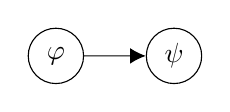
\begin{tikzpicture}
% Define styles
\tikzstyle{node} = [rounded rectangle, draw, fill=white, text centered, minimum height=2em]
% Define nodes
\node[node] (phi) at (0,0) {$\phi$};
\node[node] (psi) at (1.5,0) {$\psi$};
% Connect the nodes
\draw[->] (phi) -- (psi);
\end{tikzpicture}
\caption{Bayesian Network structure for $\psi = \phi$ and $\psi = \neg \phi$}
\end{figure}


\begin{figure}[h]
\centering
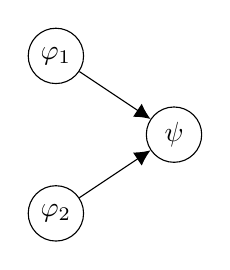
\begin{tikzpicture}
% Define styles
\tikzstyle{node} = [rounded rectangle, draw, fill=white, text centered, minimum height=2em]
% Define nodes
\node[node] (phi1) at (0,0) {$\phi_1$};
\node[node] (phi2) at (0,-2) {$\phi_2$};
\node[node] (psi) at (1.5,-1) {$\psi$};
% Connect the nodes
\draw[->] (phi1) -- (psi);
\draw[->] (phi2) -- (psi);
\end{tikzpicture}
\caption{Bayesian Network structure for $\psi = \phi_1 \land \phi_2$ and $\psi = \phi_1 \lor \phi_2$}
\end{figure}


\begin{figure}[h]
\centering
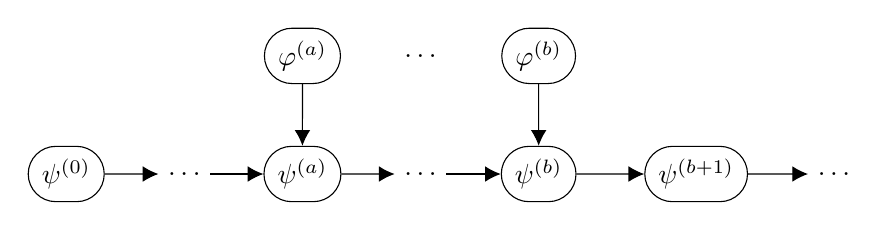
\begin{tikzpicture}
% Define styles
\tikzstyle{node} = [rounded rectangle, draw, fill=white, text centered, minimum height=2em]
% Define nodes
\node[node] (psi_0) at (0,0) {$\psi^{(0)}$};
\node (ldots0) at (1.5,0) {$\ldots$};
\node[node] (psi_a) at (3,0) {$\psi^{(a)}$};
\node[node] (phi_a) at (3,1.5) {$\phi^{(a)}$};
\node (ldots1) at (4.5,0) {$\ldots$};
\node (ldots2) at (4.5,1.5) {$\ldots$};
\node[node] (psi_b) at (6,0) {$\psi^{(b)}$};
\node[node] (phi_b) at (6,1.5) {$\phi^{(b)}$};
\node[node] (psi_b+1) at (8,0) {$\psi^{(b+1)}$};
\node (ldots3) at (9.75,0) {$\ldots$};
% Connect the nodes
\draw[->] (psi_0) -- (ldots0);
\draw[->] (ldots0) -- (psi_a);
\draw[->] (psi_a) -- (ldots1);
\draw[->] (ldots1) -- (psi_b);
\draw[->] (psi_b) -- (psi_b+1);
\draw[->] (psi_b+1) -- (ldots3);
\draw[->] (phi_a) -- (psi_a);
\draw[->] (phi_b) -- (psi_b);
\end{tikzpicture}
\caption{Bayesian Network structure for $\psi = \mathcal{F}_{[a,b]} \phi$ and $\psi = \mathcal{G}_{[a,b]} \phi$}
\end{figure}


\begin{figure}[h]
\centering
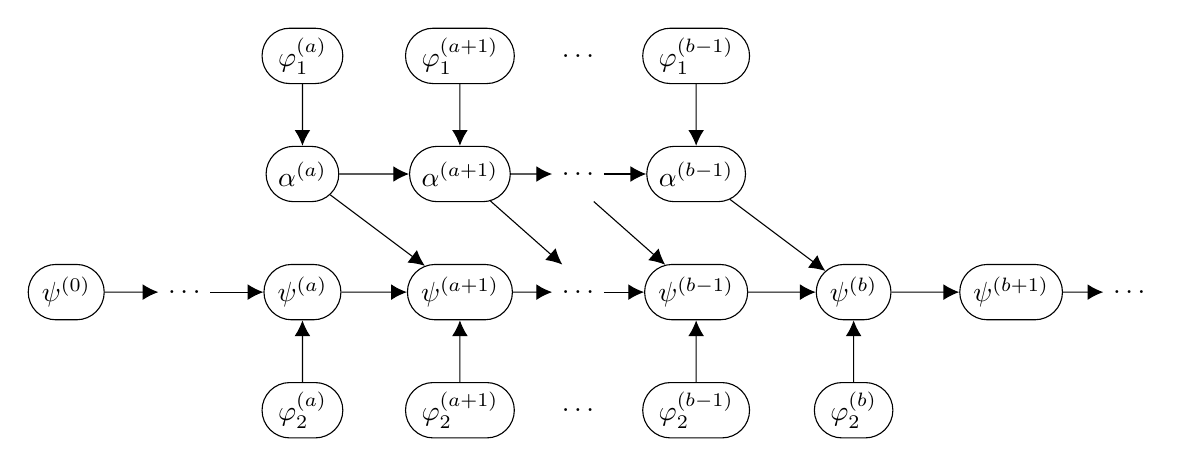
\begin{tikzpicture}
% Define styles
\tikzstyle{node} = [rounded rectangle, draw, fill=white, text centered, minimum height=2em]
% Define nodes
\node[node] (psi_0) at (0,0) {$\psi^{(0)}$};
\node (psi_ldots0) at (1.5,0) {$\ldots$};
\node[node] (psi_a) at (3,0) {$\psi^{(a)}$};
\node[node] (psi_a+1) at (5,0) {$\psi^{(a+1)}$};
\node (psi_ldots1) at (6.5,0) {$\ldots$};
\node[node] (psi_b-1) at (8,0) {$\psi^{(b-1)}$};
\node[node] (psi_b) at (10,0) {$\psi^{(b)}$};
\node[node] (psi_b+1) at (12,0) {$\psi^{(b+1)}$};
\node (psi_ldots2) at (13.5,0) {$\ldots$};
\node[node] (alpha_a) at (3,1.5) {$\alpha^{(a)}$};
\node[node] (alpha_a+1) at (5,1.5) {$\alpha^{(a+1)}$};
\node (alpha_ldots1) at (6.5,1.5) {$\ldots$};
\node[node] (alpha_b-1) at (8,1.5) {$\alpha^{(b-1)}$};
\node[node] (phi1_a) at (3,3) {$\phi_1^{(a)}$};
\node[node] (phi1_a+1) at (5,3) {$\phi_1^{(a+1)}$};
\node (phi1_ldots1) at (6.5,3) {$\ldots$};
\node[node] (phi1_b-1) at (8,3) {$\phi_1^{(b-1)}$};
\node[node] (phi2_a) at (3,-1.5) {$\phi_2^{(a)}$};
\node[node] (phi2_a+1) at (5,-1.5) {$\phi_2^{(a+1)}$};
\node (phi2_ldots1) at (6.5,-1.5) {$\ldots$};
\node[node] (phi2_b-1) at (8,-1.5) {$\phi_2^{(b-1)}$};
\node[node] (phi2_b) at (10,-1.5) {$\phi_2^{(b)}$};

% Connect the nodes
\draw[->] (psi_0) -- (psi_ldots0);
\draw[->] (psi_ldots0) -- (psi_a);
\draw[->] (psi_a) -- (psi_a+1);
\draw[->] (psi_a+1) -- (psi_ldots1);
\draw[->] (psi_ldots1) -- (psi_b-1);
\draw[->] (psi_b-1) -- (psi_b);
\draw[->] (psi_b) -- (psi_b+1);
\draw[->] (psi_b+1) -- (psi_ldots2);
\draw[->] (alpha_a) -- (psi_a+1);
\draw[->] (alpha_a+1) -- (6.3,0.35);
\draw[->] (6.7,1.15) -- (psi_b-1);
\draw[->] (alpha_b-1) -- (psi_b);
\draw[->] (alpha_a) -- (alpha_a+1);
\draw[->] (alpha_a+1) -- (alpha_ldots1);
\draw[->] (alpha_ldots1) -- (alpha_b-1);
\draw[->] (phi1_a) -- (alpha_a);
\draw[->] (phi1_a+1) -- (alpha_a+1);
\draw[->] (phi1_b-1) -- (alpha_b-1);
\draw[->] (phi2_a) -- (psi_a);
\draw[->] (phi2_a+1) -- (psi_a+1);
\draw[->] (phi2_b-1) -- (psi_b-1);
\draw[->] (phi2_b) -- (psi_b);

\end{tikzpicture}
\caption{Bayesian Network structure for $\psi = \phi_1 \mathcal{U}_{[a,b]} \phi_2$}
\end{figure}

\begin{figure}[h]
\centering
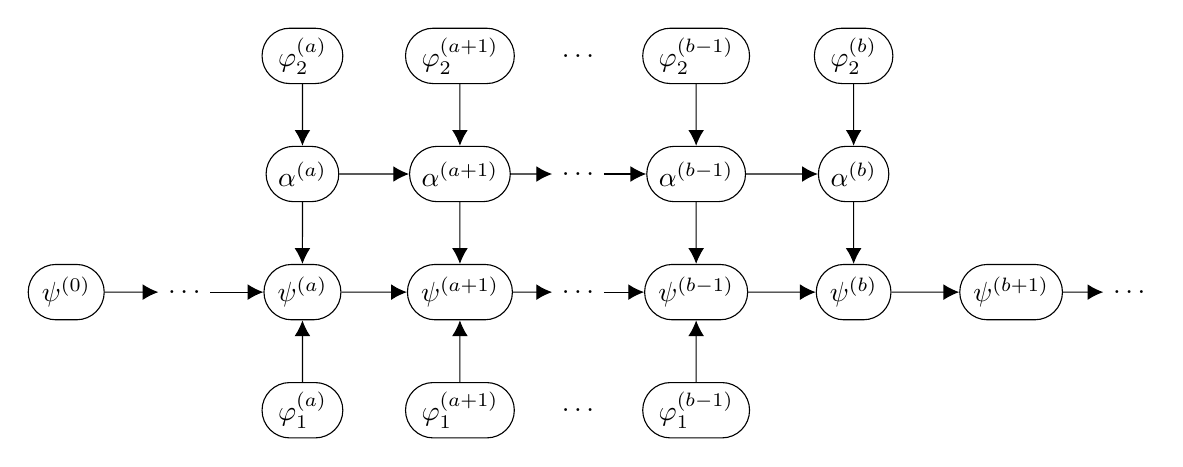
\begin{tikzpicture}
% Define styles
\tikzstyle{node} = [rounded rectangle, draw, fill=white, text centered, minimum height=2em]
% Define nodes
\node[node] (psi_0) at (0,0) {$\psi^{(0)}$};
\node (psi_ldots0) at (1.5,0) {$\ldots$};
\node[node] (psi_a) at (3,0) {$\psi^{(a)}$};
\node[node] (psi_a+1) at (5,0) {$\psi^{(a+1)}$};
\node (psi_ldots1) at (6.5,0) {$\ldots$};
\node[node] (psi_b-1) at (8,0) {$\psi^{(b-1)}$};
\node[node] (psi_b) at (10,0) {$\psi^{(b)}$};
\node[node] (psi_b+1) at (12,0) {$\psi^{(b+1)}$};
\node (psi_ldots2) at (13.5,0) {$\ldots$};
\node[node] (alpha_a) at (3,1.5) {$\alpha^{(a)}$};
\node[node] (alpha_a+1) at (5,1.5) {$\alpha^{(a+1)}$};
\node (alpha_ldots1) at (6.5,1.5) {$\ldots$};
\node[node] (alpha_b-1) at (8,1.5) {$\alpha^{(b-1)}$};
\node[node] (alpha_b) at (10,1.5) {$\alpha^{(b)}$};
\node[node] (phi2_a) at (3,3) {$\phi_2^{(a)}$};
\node[node] (phi2_a+1) at (5,3) {$\phi_2^{(a+1)}$};
\node (phi2_ldots1) at (6.5,3) {$\ldots$};
\node[node] (phi2_b-1) at (8,3) {$\phi_2^{(b-1)}$};
\node[node] (phi2_b) at (10,3) {$\phi_2^{(b)}$};
\node[node] (phi1_a) at (3,-1.5) {$\phi_1^{(a)}$};
\node[node] (phi1_a+1) at (5,-1.5) {$\phi_1^{(a+1)}$};
\node (phi1_ldots1) at (6.5,-1.5) {$\ldots$};
\node[node] (phi1_b-1) at (8,-1.5) {$\phi_1^{(b-1)}$};
% Connect the nodes
\draw[->] (psi_0) -- (psi_ldots0);
\draw[->] (psi_ldots0) -- (psi_a);
\draw[->] (psi_a) -- (psi_a+1);
\draw[->] (psi_a+1) -- (psi_ldots1);
\draw[->] (psi_ldots1) -- (psi_b-1);
\draw[->] (psi_b-1) -- (psi_b);
\draw[->] (psi_b) -- (psi_b+1);
\draw[->] (psi_b+1) -- (psi_ldots2);
\draw[->] (alpha_a) -- (psi_a);
\draw[->] (alpha_a+1) -- (psi_a+1);
\draw[->] (alpha_b-1) -- (psi_b-1);
\draw[->] (alpha_b) -- (psi_b);
\draw[->] (phi2_a) -- (alpha_a);
\draw[->] (phi2_a+1) -- (alpha_a+1);
\draw[->] (phi2_b-1) -- (alpha_b-1);
\draw[->] (phi2_b) -- (alpha_b);
\draw[->] (phi1_a) -- (psi_a);
\draw[->] (phi1_a+1) -- (psi_a+1);
\draw[->] (phi1_b-1) -- (psi_b-1);
\draw[->] (alpha_a) -- (alpha_a+1);
\draw[->] (alpha_a+1) -- (alpha_ldots1);
\draw[->] (alpha_ldots1) -- (alpha_b-1);
\draw[->] (alpha_b-1) -- (alpha_b);


\end{tikzpicture}
\caption{Bayesian Network structure for $\psi = \phi_1 \mathcal{R}_{[a,b]} \phi_2$}
\end{figure}

\newpage
\section{Evaluation}

\subsection{Datasets}

{\footnotesize
\centering
\begin{tabular}{llrrr}
Dataset            & Generating Formula                                         & \begin{tabular}[c]{@{}l@{}}Formula\\ Size\end{tabular} & \begin{tabular}[c]{@{}l@{}}Num.\\ Variables\end{tabular} & \begin{tabular}[c]{@{}l@{}}Avg. Trace\\ Length\end{tabular} \\
basic\_future      & $\mathcal{F}_{[0,10]}(p_0 \lor p_1)$                                         & 4                                                      & 2                                                         & 14.9                                                        \\
basic\_global      & $\mathcal{G}_{[0,10]}(p_0 \land p_1 \land \neg p_2)$                                   & 7                                                      & 3                                                         & 14.6                                                        \\
basic\_release     & $p_0 \mathcal{R}_{[0,10]}\ p_2$                                            & 3                                                      & 3                                                         & 14.0                                                        \\
basic\_until       & $p_1 \mathcal{U}_{[0,10]}\ p_2$                                            & 3                                                      & 3                                                         & 14.0                                                        \\
fmsd17\_formula1   & $\mathcal{G}_{[0,10]}\neg (\neg p_0 \land \neg (p_1 \mathcal{U}_{[0,10]}\ p_0))$                         & 9                                                      & 2                                                         & 24.0                                                        \\
fmsd17\_formula2   & $\mathcal{G}_{[0,99]}\neg (p_6 \land \neg ((\neg p_2 \land \neg p_3 \land \neg p_4) \mathcal{U}_{[0,99]}\ p_5))$     & 15                                                     & 7                                                         & 23.9                                                        \\
fmsd17\_formula3   & $\mathcal{G}_{[0,99]}(p_4 \land p_5 \land p_6)$                                   & 6                                                      & 7                                                         & 14.0                                                        \\
nasa-atc\_formula1 & $\mathcal{G}_{[0,10]}\neg (\neg p_0 \land \neg (p_1 \mathcal{U}_{[0,10]}\ p_0))$                         & 9                                                      & 2                                                         & 23.9                                                        \\
nasa-atc\_formula2 & $\mathcal{G}_{[0,99]}\neg (p_6 \land \neg ((\neg p_2 \land \neg p_3 \land \neg p_4) \mathcal{U}_{[0,99]}\ p_5))$     & 15                                                     & 7                                                         & 23.9                                                        \\
rv14\_formula1     & $\mathcal{G}_{[0,99]}\neg (p_1 \land (\texttt{tt} \mathcal{U}_{[0,30]}\ p_0) \land (\texttt{tt} \mathcal{U}_{[0,99]}\ p_2))$ & 11                                                     & 3                                                         & 14.0                                                        \\
rv14\_formula2     & $\mathcal{G}_{[0,99]}\neg (\neg p_0 \land \neg (p_1 \mathcal{U}_{[0,30]}\ p_0))$                      & 9                                                      & 2                                                         & 14.1                                                       
\end{tabular}
}

\subsection{Results}
\subsubsection {Beam Search}

\footnotesize
\begin{center}
\begin{tabular}{llrrr}
Dataset                             & Best Formula(s) Found                                                                                   & \begin{tabular}[c]{@{}l@{}}Formula\\ Size\end{tabular} & \begin{tabular}[c]{@{}l@{}}Compute\\ Time (s)\end{tabular} & \begin{tabular}[c]{@{}l@{}}Formula\\ Accuracy\end{tabular} \\
basic\_future                       & $\mathcal{F}_{[0,10]}(p_1 \lor p_0)$                                                                                 & 4                                                      & 0.1                                                        & 100\%                                                      \vspace{0.5em}\\
basic\_global                       & $\mathcal{G}_{[0,10]}(p_0 \land p_1 \land \neg p_2)$                                                                           & 7                                                      & 0.2                                                        & 100\%                                                      \vspace{0.5em}\\
basic\_release                      & $p_0 \mathcal{R}_{[0,10]}\ p_2$                                                                                    & 3                                                      & 0.2                                                        & 100\%                                                      \vspace{0.5em}\\
basic\_until                        & $p_1 \mathcal{U}_{[0,10]}\ p_2$                                                                                    & 3                                                      & 0.2                                                        & 100\%                                                      \vspace{0.5em}\\
fmsd17\_formula1                    & $\mathcal{G}_{[0,10]}(p_1 \mathcal{U}_{[0,15]}\ p_0)$                                                                           & 4                                                      & 1.4                                                        & 100\%                                                      \vspace{0.5em}\\
\multirow{2}{*}{fmsd17\_formula2}   & $\mathcal{G}_{[0,10]}(((\neg p_6 \lor p_5) \mathcal{U}_{[0,15]}\ (\neg p_2 \land \neg p_3)) \lor \neg p_6 \lor p_5)$                                             & 16                                                     & 13.3                                                       & 98.2\%\ \ \\
                                    & \begin{tabular}[c]{@{}l@{}}$\mathcal{G}_{[0,10]}((\neg p_6 \mathcal{U}_{[0,5]}\ p_5) \lor \neg p_6 \lor \neg p_4)$ \\ \hspace{2em}$\mathcal{R}_{[0,10]}\ \mathcal{G}_{[0,10]}(((\neg p_6 \lor p_5) \mathcal{U}_{[0,5]}\ (\neg p_2 \land \neg p_3)) \lor \neg p_6 \lor p_5)$\end{tabular} & 28                                                     & 138.9                                                      & 99.4\%                                                     \vspace{0.5em}\\
fmsd17\_formula3                    & $\mathcal{G}_{[0,10]}(p_4 \land p_5 \land p_6)$                                                                            & 6                                                      & 19.4                                                       & 100\%                                                      \vspace{0.5em}\\
nasa-atc\_formula1                  & $\mathcal{G}_{[0,10]}(p_1 \mathcal{U}_{[0,10]}\ p_0)$                                                                           & 4                                                      & 2.3                                                        & 100\%                                                      \vspace{0.5em}\\
\multirow{2}{*}{nasa-atc\_formula2} & $\mathcal{G}_{[0,10]}(((\neg p_6 \lor p_5) \mathcal{U}_{[0,10]}\ (\neg p_2 \land \neg p_3)) \lor \neg p_6 \lor p_5)$                                             & 16                                                     & 21.8                                                       & 97.6\%\ \                                                      \\
                                    &    \begin{tabular}[c]{@{}l@{}}$\mathcal{G}_{[0,10]}(((\neg p_6 \lor \neg p_4) \mathcal{U}_{[0,5]}\ p_5) \lor \neg p_6)$ \\ \hspace{2em} $\mathcal{R}_{[0,10]}\ \mathcal{G}_{[0,10]}((\neg p_2 \land \lor p      _3) \mathcal{U}_{[0,5]} (\neg p_6 \lor p_5))$\end{tabular}                  & 23                                                     & 4022.4                                                     & 99.2\%                                                     \vspace{0.5em}\\
\multirow{2}{*}{rv14\_formula1}     & $\mathcal{G}_{[0,10]}((p_1 \mathcal{R}_{[0,5]}\ (\neg p_2 \lor \neg p_0)) \lor \neg p_1)$                                                           & 11                                                     & 2.3                                                        & 100\% \                                                     \\
                                    & $\mathcal{G}_{[0,10]}(\neg p_2 \lor \neg p_1 \lor \neg p_0)$                                                                         & 9                                                      & 3.3                                                        & 100\%                                                      \vspace{0.5em}\\
rv14\_formula2                      & $\mathcal{G}_{[0,10]}((p_0 \land p_1) \mathcal{U}_{[0,5]}\ p_0)$                                                                     & 6                                                      & 0.8                                                        & 100\%\ \                                                      
\end{tabular}
\end{center}


\subsubsection {Template Driven Search}
\footnotesize
\begin{center}
\begin{tabular}{llrrr}
Dataset                             & Best Formula(s) Found                                                                                   & \begin{tabular}[c]{@{}l@{}}Formula\\ Size\end{tabular} & \begin{tabular}[c]{@{}l@{}}Compute\\ Time (s)\end{tabular} & \begin{tabular}[c]{@{}l@{}}Formula\\ Accuracy\end{tabular} \\
basic\_future                       & $\mathcal{F}_{[0,10]}(p_1 \lor p_0)$                                                                                 & 4                                                      & 1.0                                                        & 100\%                                                      \vspace{0.5em}\\
basic\_global                       & $\mathcal{G}_{[0,10]}(p_0 \land p_1 \land \neg p_2)$                                                                           & 7                                                      & 7.9                                                        & 100\%                                                      \vspace{0.5em}\\
basic\_release                      & $p_0 \mathcal{R}_{[0,10]}\ p_2$                                                                                    & 3                                                      & 1.0                                                        & 100\%                                                      \vspace{0.5em}\\
basic\_until                        & $p_1 \mathcal{U}_{[0,10]}\ p_2$                                                                                    & 3                                                      & 1.8                                                        & 100\%                                                      \vspace{0.5em}\\                                            
\end{tabular}
\end{center}
\section{Conclusion}


\section{Statement of Contributions}
% To ensure that each team member gets credit for his or her
% contributions, the final report should include a statement of contributions that explicitly
% identifies the contributions of each team member and a statement that every team
% member concurs with the contents of the report.
\

Throughout this project, all team members have consistently collaborated, from the initial brainstorming of approaches to discussions of challenges encountered and potential solutions. The project's workload was divided in a manner that allowed each team member to leverage their expertise and interests to explore the feasibility of a different approach. The notable contributions of each team member are outlined below.



\textit{Zili Wang} -- 

\textit{Luke Marzen} -- Contributed the beam search based solution for the MLTL-inference problem. Wrote a working multi-threaded beam search implementation in C++ and evaluated its performance. Implemented the Quine-McCluskey algorithm to generate simplified DNF boolean functions.

\textit{Nhan Tran} -- 

\textit{Swaminathan Jayaraman} -- Contributed the template drive search approach for the MLTL formula synthesis. Explored and implemented a form of Counterexample Guided Inductive Synthesis (CEGIS) logic in python through a  combination of inductive synthesis, heuristic scoring, iterative deepening search and abstraction refinement.


\newpage
\bibliographystyle{splncs04}
\bibliography{Citations}
\end{document}
